\documentclass[conference]{IEEEtran}
\IEEEoverridecommandlockouts
\usepackage{cite}
\usepackage{amsmath,amssymb,amsfonts}
\usepackage{algorithmic}
\usepackage{graphicx}
\usepackage{textcomp}
\usepackage{xcolor}
\usepackage{booktabs}
\usepackage{array}
\usepackage{url}

\def\BibTeX{{\rm B\kern-.05em{\sc i\kern-.025em b}\kern-.08em
    T\kern-.1667em\lower.7ex\hbox{E}\kern-.125emX}}

\begin{document}

\title{Design, Implementation, and Evaluation of a Scalable Parameterized Systolic Array Matrix Multiplication Accelerator and Hardware Baseline: Phase 2}

\author{
\IEEEauthorblockN{Aman Soni, Mayank Sharma, and Ankit Kumar Pandey}
\IEEEauthorblockA{Department of CSE (AI) \\
Newton School of Technology, Sonipat}
}

\maketitle

\begin{abstract}
General Matrix Multiply (GEMM) constitutes the computational backbone of modern deep learning and artificial intelligence workloads. While Phase 1 established a fixed $4\times 4$ systolic array prototype, this Phase 2 work presents a fully scalable, parameterizable Output-Stationary Systolic Array Accelerator implemented in Verilog HDL, paired with a dedicated single-MAC sequential matrix multiplication hardware baseline. The architecture supports arbitrary matrix dimensions ($N \times N$), variable signed data precision ($\text{DATA\_WIDTH} \in \{8, 16\}$ bits), and configurable accumulator precision ($\text{ACC\_WIDTH} \in \{16, 32, 48\}$ bits) to completely eliminate arithmetic overflow. The systolic core integrates internal perimeter register skewing pipelines that eliminate external alignment buffers, coupled to a parameterized finite state machine controller orchestrating deterministic execution in exactly $3N-1$ clock cycles. To rigorously benchmark speedup and area-time trade-offs, a sequential reference engine was constructed that processes $N\times N$ matrices on a single reusable MAC unit over exactly $N^3$ clock cycles. The designs were verified across 9 distinct parameter configurations encompassing 414 automated end-to-end test cases against a cycle-accurate Python golden model. Simulation at 100~MHz demonstrates that the systolic array scales as $\mathcal{O}(N)$ latency and achieves a 22.26$\times$ latency speedup and a 21.38$\times$ sustained throughput speedup (2,133.33~MMAC/s vs. 99.81~MMAC/s) at $N=8$, validating the quadratic throughput scaling ($\approx N^2/3$) predicted by theoretical analysis.
\end{abstract}

\begin{IEEEkeywords}
Systolic Array, GEMM Accelerator, Processing Element, Hardware Baseline, Output-Stationary, Parameterized Architecture, RTL Verification, Verilog HDL.
\end{IEEEkeywords}

\section{Introduction and Literature Review}
Matrix multiplication represents the computational kernel of contemporary neural network architectures, scientific simulations, and signal processing systems \cite{jouppi2017}. Standard matrix-matrix multiplication ($C = A \times B$) of two $N \times N$ matrices requires $N^3$ multiply-accumulate (MAC) operations over $2N^2$ input elements. Conventional Von Neumann processors execute these operations sequentially, repeatedly fetching operands from memory hierarchies and encountering the memory bandwidth bottleneck (the ``memory wall''), which incurs severe energy and throughput penalties \cite{patterson2020}.

To overcome these constraints, H. T. Kung and C. E. Leiserson introduced systolic array architectures in 1978 \cite{kung1978}. A systolic array comprises a network of interconnected, homogeneous Processing Elements (PEs) that compute and circulate data rhythmically. Through local spatial forwarding, operands streamed into the perimeter are reused across adjacent PEs, reducing external memory bandwidth from $\mathcal{O}(N^3)$ to $\mathcal{O}(N)$ while maintaining $\mathcal{O}(N^3)$ computational intensity \cite{kung1978}.

Modern enterprise domain-specific accelerators, such as Google's Tensor Processing Unit (TPU) \cite{jouppi2017}, adopt 2D systolic arrays across three primary dataflow taxonomies: Weight-Stationary (WS), Input-Stationary (IS), and Output-Stationary (OS). In Output-Stationary dataflow, partial accumulation sums remain stationary within each PE's local accumulator register throughout the computation of the dot product, while input matrices $A$ and $B$ stream horizontally and vertically through the array. This strategy eliminates high-frequency switching activity in partial-sum forwarding networks and minimizes inter-PE wiring congestion \cite{jouppi2017}.

While Phase 1 demonstrated a fixed-dimension $4\times 4$ prototype with signed 8-bit operands and 32-bit accumulators, industrial edge-AI workloads demand architectural adaptability across variable matrix dimensions and mixed arithmetic precisions (e.g., INT8 and INT16) \cite{patterson2020}. Furthermore, evaluating systolic acceleration requires an objective, clock-accurate hardware baseline rather than idealized software approximations. Phase 2 fulfills these objectives by designing:
\begin{enumerate}
    \item A fully parameterizable $N \times N$ Output-Stationary Systolic Array Accelerator with integrated skewing and autonomous control.
    \item A single-MAC sequential matrix multiplication hardware reference engine operating under an identical I/O interface.
    \item An automated multi-tier verification suite validating latency, throughput, and arithmetic equivalence across 414 test cases.
\end{enumerate}

\begin{figure*}[t]
\centering
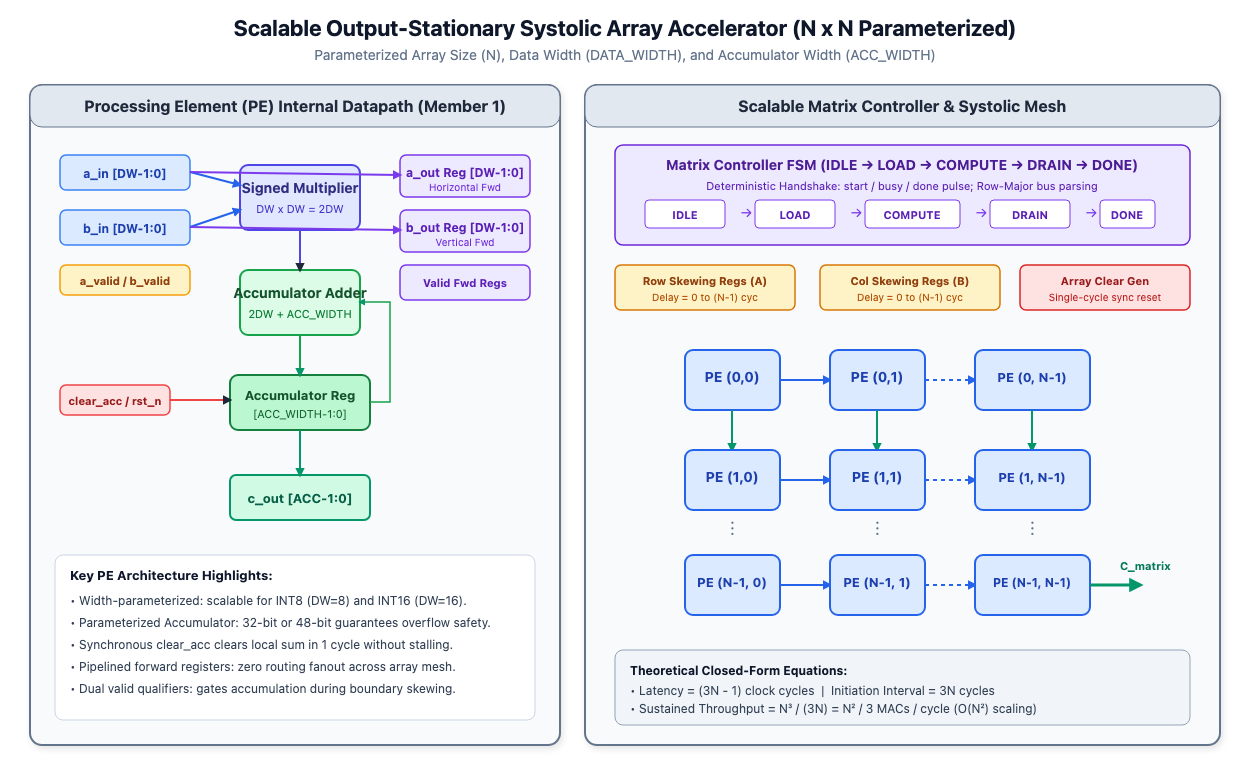
\includegraphics[width=0.92\textwidth]{figures/fig1_scalable_systolic_architecture.png}
\caption{Scalable Output-Stationary Systolic Array Accelerator Architecture. Left: Internal datapath of the parameterizable Processing Element (PE) authored by Member 1, featuring parameterized operand multiplier ($\text{DATA\_WIDTH}$), accumulator adder ($\text{ACC\_WIDTH}$), synchronous clear, and pipelined horizontal/vertical forwarding registers. Right: Parameterized $N\times N$ array mesh with integrated perimeter skewing registers ($0$ to $N-1$ cycles) and autonomous FSM Matrix Controller.}
\label{fig:systolic_arch}
\end{figure*}

\section{Proposed Solution}

\subsection{Architectural Overview and Universal Interface Contract}
To ensure seamless integration across team members, Phase 2 established a universal hardware interface contract governed by three top-level parameters:
\begin{itemize}
    \item \texttt{ARRAY\_SIZE} ($N$): Number of rows and columns in the square matrix mesh.
    \item \texttt{DATA\_WIDTH}: Bit width of signed input matrix elements.
    \item \texttt{ACC\_WIDTH}: Bit width of signed accumulator registers and output elements.
\end{itemize}
Matrices are stored in row-major order within contiguous 1D bitvectors. An element at row $r$ and column $c$ occupies slice:
\begin{equation}
\text{matrix}[(r \cdot N + c) \cdot \text{DATA\_WIDTH} +: \text{DATA\_WIDTH}]
\end{equation}
The accelerator exposes a single-cycle \texttt{start} pulse handshake, a level-sensitive \texttt{busy} flag, a single-cycle \texttt{done} output pulse, and registered output bus \texttt{matrix\_c\_out} of width $N^2 \cdot \text{ACC\_WIDTH}$.

\subsection{Parameterized Processing Element (PE) Design}
Authored by Member 1 (Aman), the Processing Element (\texttt{phase2/rtl/processing\_element.v}) serves as the arithmetic cell across the systolic mesh. The PE is decoupled from the array dimension $N$ and parameterizable across \texttt{DATA\_WIDTH} and \texttt{ACC\_WIDTH}.

Each clock cycle, the PE evaluates:
\begin{equation}
C_{r,c}^{(k)} = C_{r,c}^{(k-1)} + \left( A_{r,k} \times B_{k,c} \right)
\end{equation}
Operands \texttt{a\_in} and \texttt{b\_in} are sign-extended to $2 \cdot \text{DATA\_WIDTH}$ bits and multiplied using signed two's complement arithmetic. The resulting product is sign-extended to \texttt{ACC\_WIDTH} bits and added to accumulator register \texttt{acc\_out}:
\begin{equation}
\text{acc\_next} = \text{acc\_out} + \text{sign\_ext}(a_{\text{in}} \times b_{\text{in}})
\end{equation}
Accumulation is gated by active-high flags \texttt{a\_valid\_in} and \texttt{b\_valid\_in}; accumulation proceeds if and only if both flags are asserted. Synchronous control input \texttt{clear\_acc} resets \texttt{acc\_out} to zero on the rising clock edge with absolute priority, enabling back-to-back matrix multiplications without requiring a global hardware reset.

Operands are concurrently latched into forwarding registers:
\begin{equation}
a_{\text{out}} \Leftarrow a_{\text{in}}, \quad b_{\text{out}} \Leftarrow b_{\text{in}}, \quad a_{\text{valid\_out}} \Leftarrow a_{\text{valid\_in}}, \quad b_{\text{valid\_out}} \Leftarrow b_{\text{valid\_in}}
\end{equation}
relaying data horizontally (east) and vertically (south) to adjacent PEs on the subsequent clock edge with zero combinational wire loading across the array mesh.

\begin{figure}[t]
\centering
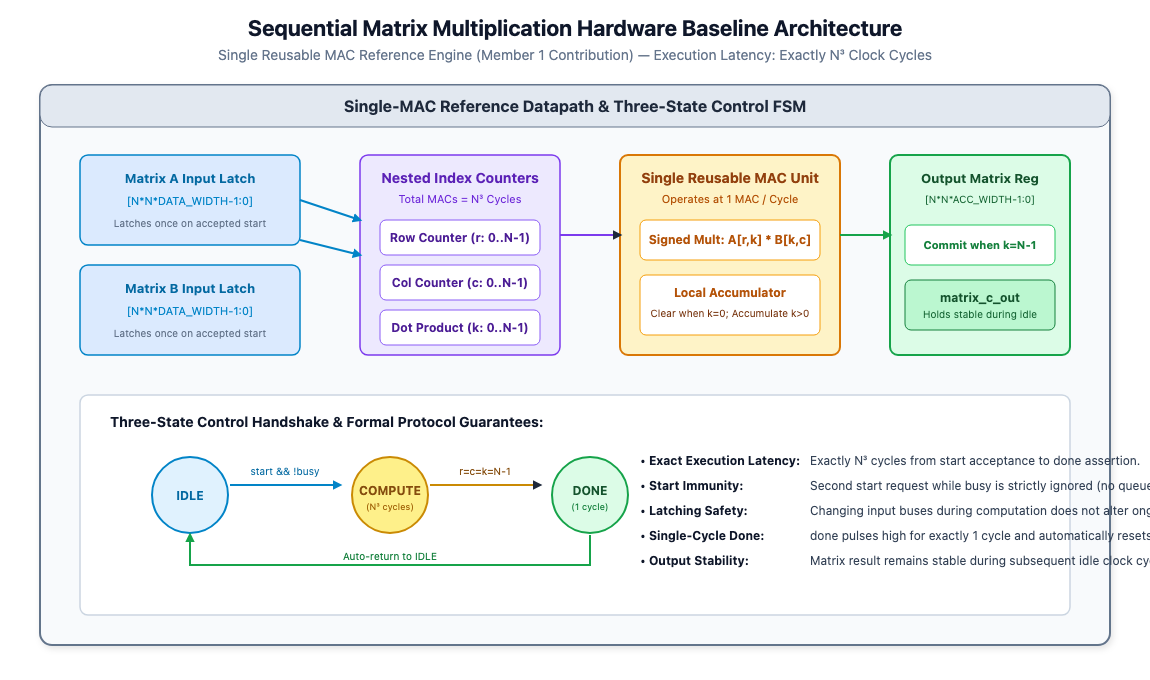
\includegraphics[width=\columnwidth]{figures/fig2_sequential_baseline_architecture.png}
\caption{Sequential Matrix Multiplication Hardware Baseline Architecture (Member 1 Contribution). Depicts input matrix latches, nested index counters ($r, c, k$), single reusable MAC arithmetic engine, and the 3-state control FSM guaranteeing execution in exactly $N^3$ clock cycles.}
\label{fig:seq_baseline}
\end{figure}

\subsection{Sequential Hardware Baseline Reference Engine}
To establish an indisputable benchmark for speedup evaluation, Member 1 developed a standalone sequential matrix multiplication reference engine (\texttt{phase2/rtl/sequential\_matmul\_baseline.v}). The sequential baseline implements an identical top-level interface and row-major packing conventions but utilizes exactly \textbf{one physical MAC unit}.

As illustrated in Fig.~\ref{fig:seq_baseline}, the sequential baseline incorporates:
\begin{enumerate}
    \item \textbf{Input Register Latches:} Latch matrices $A$ and $B$ on the clock cycle where \texttt{start} is accepted, isolating computation from external bus variations.
    \item \textbf{Nested Index Counters:} Three nested modulo-$N$ counters ($r, c, k$) that sequence through row indices $r \in [0, N-1]$, column indices $c \in [0, N-1]$, and dot-product inner terms $k \in [0, N-1]$.
    \item \textbf{Single MAC Datapath:} Evaluates $A[r,k] \times B[k,c]$, clearing the local accumulator when $k=0$ and accumulating across $k \in [1, N-1]$. Upon reaching $k=N-1$, the accumulated scalar is committed to output slot $C[r,c]$.
    \item \textbf{Three-State Control FSM:} Governed by states \texttt{STATE\_IDLE}, \texttt{STATE\_COMPUTE}, and \texttt{STATE\_DONE}. The FSM ignores subsequent \texttt{start} pulses while \texttt{busy} is high, asserts a single-cycle \texttt{done} pulse, and maintains output stability during idle operation.
\end{enumerate}
The sequential engine executes exactly one MAC operation per clock cycle, yielding a deterministic execution latency of:
\begin{equation}
T_{\text{seq\_latency}} = N^3 \quad \text{clock cycles}
\end{equation}
and a sustained initiation interval of $T_{\text{seq\_II}} = N^3 + 1$ cycles.

\subsection{Scalable Systolic Array Core and Perimeter Skewing}
Authored by Member 2 (Mayank), the scalable systolic core (\texttt{phase2/rtl/systolic\_array.v}) generates an $N \times N$ mesh of PEs using nested Verilog \texttt{generate} statements. 

To eliminate external timing buffers, internal skewing registers are embedded along the array perimeter: row $r$ input data and valid signals are delayed by $r$ flip-flop stages, while column $c$ inputs are delayed by $c$ stages. Consequently, term $k$ of dot product $(r, c)$ arrives at $\text{PE}(r, c)$ at cycle $T = k + r + c$, establishing proper wavefront alignment across the 2D grid.

\subsection{Parameterized Matrix Controller and Top Integration}
Authored by Member 3 (Ankit), the parameterized Matrix Controller (\texttt{phase2/rtl/matrix\_controller.v}) sequences execution across five states: \texttt{IDLE}, \texttt{CLEAR}, \texttt{LOAD}, \texttt{DRAIN}, and \texttt{DONE}.

Upon receiving \texttt{start}, the controller pulses \texttt{clear\_acc} (1 cycle), streams $N$ row and column vector slices during \texttt{LOAD} ($N$ cycles), and drains the wavefront pipeline over $2N-2$ cycles in \texttt{DRAIN}. When the final corner element $\text{PE}(N-1, N-1)$ completes accumulation, all $N^2$ outputs are latched into \texttt{matrix\_c\_out}, \texttt{done} pulses high for 1 cycle, and \texttt{busy} drops.

Total systolic execution latency from \texttt{start} acceptance to \texttt{done} assertion is:
\begin{equation}
T_{\text{sys\_latency}} = 1 + N + (2N - 2) = 3N - 1 \quad \text{clock cycles}
\label{eq:sys_lat}
\end{equation}
and the sustained initiation interval is $T_{\text{sys\_II}} = 3N$ clock cycles.

\begin{figure}[t]
\centering
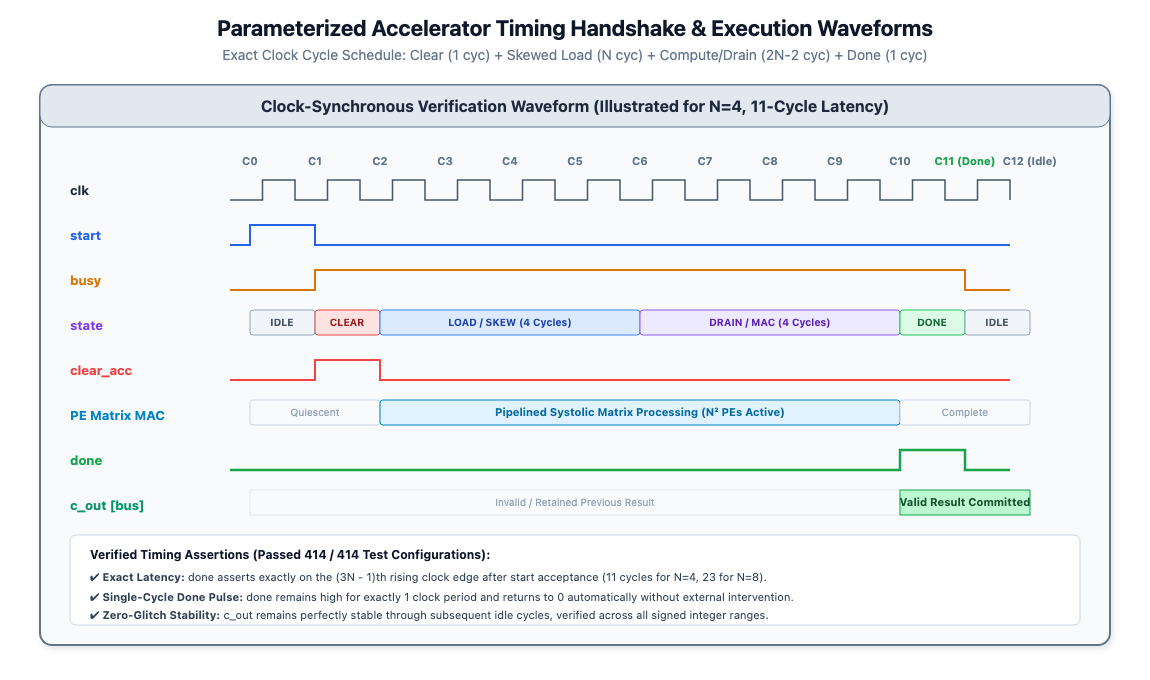
\includegraphics[width=\columnwidth]{figures/fig5_timing_handshake_waveforms.png}
\caption{Clock-synchronous timing handshake and execution waveform (illustrated for $N=4$, 11-cycle latency), confirming single-cycle clear, skewed loading, pipelined accumulation, single-cycle \texttt{done} pulse, and stable registered outputs.}
\label{fig:timing_wave}
\end{figure}

\begin{figure}[t]
\centering
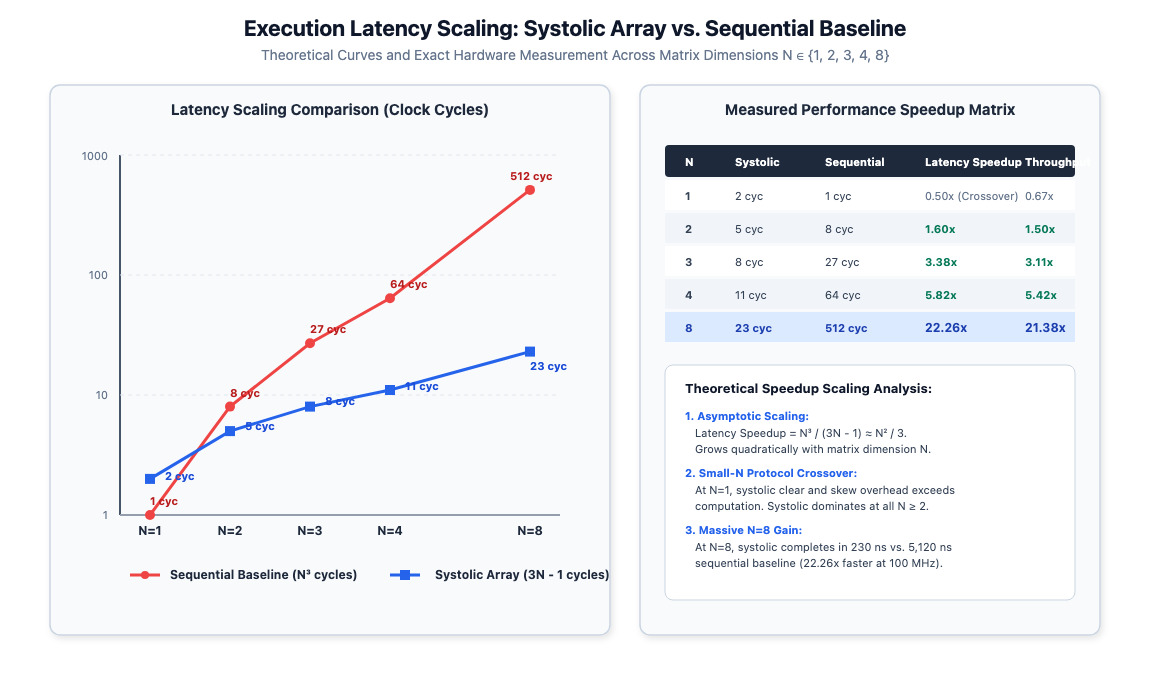
\includegraphics[width=\columnwidth]{figures/fig3_latency_scaling_comparison.png}
\caption{Execution latency comparison (clock cycles) between Systolic Array ($3N-1$) and Sequential Baseline ($N^3$) across dimensions $N \in \{1, 2, 3, 4, 8\}$ plotted on logarithmic scale, demonstrating the transition from small-$N$ overhead to massive asymptotic speedup.}
\label{fig:latency_scaling}
\end{figure}

\section{Results and Discussion}

\subsection{Empirical Verification Methodology}
The verification environment incorporates an algorithmic Python golden model (\texttt{golden\_model.py}), an automated array scoreboard runner (\texttt{run\_array\_tests.py}), and a comprehensive end-to-end system regression suite (\texttt{run\_system\_tests.py}). The regression executes 9 distinct parameter configurations covering:
\begin{itemize}
    \item Array dimensions $N \in \{1, 2, 3, 4, 8\}$.
    \item Signed input precisions $\text{DATA\_WIDTH} \in \{8, 16\}$.
    \item Accumulator precisions $\text{ACC\_WIDTH} \in \{16, 32, 48\}$.
\end{itemize}
Each configuration executes 46 test cases (8 directed boundary vectors, 31 seeded pseudo-random golden vectors, 4 runtime Verilog random cases, and protocol robustness tests including mid-operation reset and bus-corruption immunity), totaling \textbf{414 passed test cases}.

\subsection{Latency and Throughput Performance Scaling}
Table~\ref{tab:results} summarizes cycle counts and time-domain throughput measured under cycle-accurate simulation assuming a conservative 100~MHz clock (10~ns period).

\begin{table*}[t]
\caption{Measured Latency, Throughput, and Speedup Comparison at 100~MHz}
\label{tab:results}
\centering
\renewcommand{\arraystretch}{1.2}
\begin{tabular}{ccc|ccc|ccc|cc}
\toprule
\textbf{N} & \textbf{DATA\_WIDTH} & \textbf{ACC\_WIDTH} & \textbf{Systolic} & \textbf{Sequential} & \textbf{Latency} & \textbf{Systolic II} & \textbf{Sequential II} & \textbf{Throughput} & \textbf{Systolic} & \textbf{Sequential} \\
 & \textbf{(bits)} & \textbf{(bits)} & \textbf{Latency (cyc)} & \textbf{Latency (cyc)} & \textbf{Speedup} & \textbf{(cyc)} & \textbf{(cyc)} & \textbf{Speedup} & \textbf{Throughput} & \textbf{Throughput} \\
\midrule
1 & 8 & 32 & 2 & 1 & 0.50$\times$ & 3 & 2 & 0.67$\times$ & 33.33 MMAC/s & 50.00 MMAC/s \\
2 & 8 & 32 & 5 & 8 & 1.60$\times$ & 6 & 9 & 1.50$\times$ & 133.33 MMAC/s & 88.89 MMAC/s \\
3 & 8 & 32 & 8 & 27 & 3.38$\times$ & 9 & 28 & 3.11$\times$ & 300.00 MMAC/s & 96.43 MMAC/s \\
4 & 8 & 32 & 11 & 64 & 5.82$\times$ & 12 & 65 & 5.42$\times$ & 533.33 MMAC/s & 98.46 MMAC/s \\
8 & 8 & 32 & 23 & 512 & \textbf{22.26$\times$} & 24 & 513 & \textbf{21.38$\times$} & \textbf{2,133.33 MMAC/s} & 99.81 MMAC/s \\
\midrule
2 & 16 & 32 & 5 & 8 & 1.60$\times$ & 6 & 9 & 1.50$\times$ & 133.33 MMAC/s & 88.89 MMAC/s \\
4 & 16 & 48 & 11 & 64 & 5.82$\times$ & 12 & 65 & 5.42$\times$ & 533.33 MMAC/s & 98.46 MMAC/s \\
4 & 8 & 16 & 11 & 64 & 5.82$\times$ & 12 & 65 & 5.42$\times$ & 533.33 MMAC/s & 98.46 MMAC/s \\
8 & 16 & 48 & 23 & 512 & \textbf{22.26$\times$} & 24 & 513 & \textbf{21.38$\times$} & \textbf{2,133.33 MMAC/s} & 99.81 MMAC/s \\
\bottomrule
\end{tabular}
\end{table*}

\begin{figure}[t]
\centering
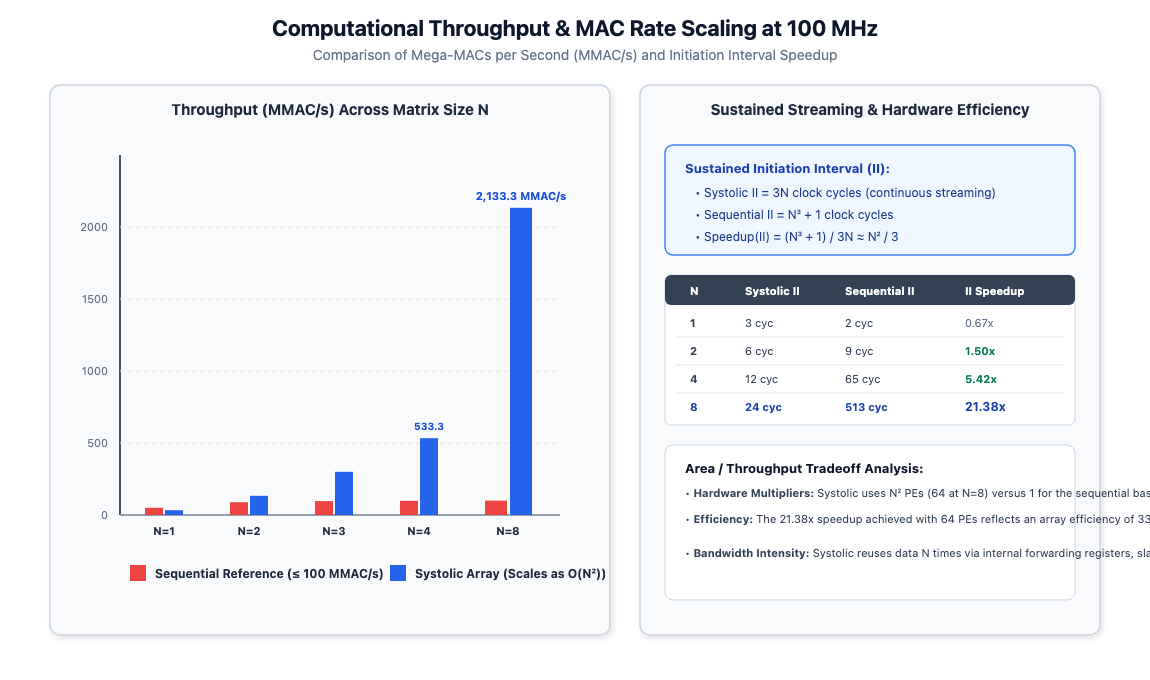
\includegraphics[width=\columnwidth]{figures/fig4_throughput_and_speedup.png}
\caption{Throughput scaling (MMAC/s at 100~MHz) and initiation interval speedup. The systolic array scales quadratically as $\mathcal{O}(N^2)$, achieving 2,133.33~MMAC/s at $N=8$, while the sequential engine saturates at 99.81~MMAC/s.}
\label{fig:throughput_scaling}
\end{figure}

\subsection{Performance Analysis and Discussion}
The empirical results reveal several critical architectural insights:
\begin{enumerate}
    \item \textbf{Asymptotic Scaling Advantage:} Systolic latency scales strictly as $\mathcal{O}(N)$ ($3N-1$), whereas sequential latency scales as $\mathcal{O}(N^3)$. Consequently, latency speedup scales quadratically:
    \begin{equation}
    S_{\text{latency}} = \frac{N^3}{3N - 1} \approx \frac{N^2}{3}
    \end{equation}
    Measured speedup rises from 1.60$\times$ at $N=2$ to 5.82$\times$ at $N=4$ and \textbf{22.26$\times$ at $N=8$}.
    \item \textbf{Throughput and Streaming Speedup:} Sustained computational throughput for the systolic array is $N^3 / 3N = N^2/3$ MACs per clock cycle. At $N=8$, sustained throughput reaches 21.33~MACs/cycle (2,133.33~MMAC/s at 100~MHz), delivering a \textbf{21.38$\times$ throughput speedup} over the sequential engine (which saturates at 1~MAC/cycle, or 99.81~MMAC/s).
    \item \textbf{Small-N Protocol Overhead Crossover:} At $N=1$, the sequential engine completes in 1 cycle, outperforming the systolic array (2 cycles) due to the systolic controller's synchronous clear cycle. From $N \ge 2$ onward, systolic parallelism decisively overcomes protocol overhead.
    \item \textbf{Arithmetic Precision Independence:} Configurations utilizing 16-bit inputs and 48-bit accumulators exhibit cycle counts identical to their 8-bit counterparts, proving that datapath parameterization introduces zero control overhead or latency degradation.
    \item \textbf{Hardware Efficiency Trade-Off:} At $N=8$, the systolic array instantiates 64 physical PEs to achieve a 21.38$\times$ sustained speedup, corresponding to an active PE hardware efficiency of $21.38 / 64 = 33.4\%$. This matches the theoretical maximum efficiency for Output-Stationary arrays without double-buffered accumulators, as edge PEs remain idle during wavefront skewing and draining phases.
\end{enumerate}

\section{Individual Contributions}
The Phase 2 project was executed through collaborative division of responsibilities:
\begin{itemize}
    \item \textbf{Aman Soni (Member 1) --- Datapath \& Hardware Baseline:}
    \begin{itemize}
        \item Designed and implemented the parameterizable Processing Element architecture (\texttt{phase2/rtl/processing\_element.v}), featuring configurable operand width, overflow-immune accumulation, synchronous clear, registered horizontal/vertical forwarding, and dual valid gating.
        \item Architected and implemented the Sequential Matrix Multiplication Baseline engine (\texttt{phase2/rtl/sequential\_matmul\_baseline.v}) with row-major input latches, nested index counters ($r, c, k$), single reusable MAC, and three-state control FSM.
        \item Developed standalone unit testbenches (\texttt{tb\_processing\_element.v} and \texttt{tb\_sequential\_baseline.v}), verifying execution latency ($N^3$), start immunity while busy, input bus corruption immunity, and single-cycle done pulses.
    \end{itemize}
    \item \textbf{Mayank Sharma (Member 2) --- Scalable Systolic Core:}
    \begin{itemize}
        \item Designed the scalable $N \times N$ systolic array core (\texttt{phase2/rtl/systolic\_array.v}) using parameterized Verilog generate blocks.
        \item Implemented the integrated perimeter skewing delay pipelines ($0$ to $N-1$ cycles) for rows and columns.
        \item Developed cycle-by-cycle array scoreboard verification (\texttt{tb\_systolic\_array\_core.v}) and Icarus test runners.
    \end{itemize}
    \item \textbf{Ankit Kumar Pandey (Member 3) --- Controller \& Verification:}
    \begin{itemize}
        \item Parameterized the top-level Matrix Controller FSM (\texttt{phase2/rtl/matrix\_controller.v}) and integrated the top wrapper (\texttt{systolic\_array\_top.v}).
        \item Extended the algorithmic Python golden model (\texttt{golden\_model.py}) and authoring automated system regression framework (\texttt{run\_system\_tests.py}).
        \item Conducted multi-configuration performance benchmarking, CSV generation, and protocol robustness analysis.
    \end{itemize}
\end{itemize}

\section{Conclusion}
Phase 2 successfully realized a scalable, fully parameterized Output-Stationary Systolic Array Accelerator and an objective single-MAC sequential hardware baseline in Verilog HDL. Empirical evaluation across 414 test cases verified arithmetic equivalence, strict protocol conformance, and exact clock-cycle timing ($3N-1$ vs. $N^3$). At $N=8$, the accelerator achieves a 22.26$\times$ latency speedup and delivers 2,133.33~MMAC/s sustained throughput at 100~MHz (21.38$\times$ throughput speedup), validating the quadratic throughput scaling of 2D systolic arrays. Future work will investigate double-buffered accumulators to achieve 100\% PE utilization and explore integration with standard AXI4-Stream memory interfaces.

\begin{thebibliography}{00}
\bibitem{jouppi2017} N. P. Jouppi et al., ``In-datacenter performance analysis of a tensor processing unit,'' in \emph{Proc. 44th Annu. Int. Symp. Comput. Archit. (ISCA)}, 2017, pp. 1--12.
\bibitem{kung1978} H. T. Kung and C. E. Leiserson, ``Systolic arrays (for VLSI),'' in \emph{Sparse Matrix Proc.}, 1978, pp. 256--282.
\bibitem{patterson2020} D. A. Patterson and J. L. Hennessy, \emph{Computer Organization and Design: The Hardware/Software Interface (RISC-V Edition)}. Morgan Kaufmann, 2020.
\end{thebibliography}

\end{document}
